
\subsection{Processing of relative clauses}
\begin{figure*}[t]
\centering
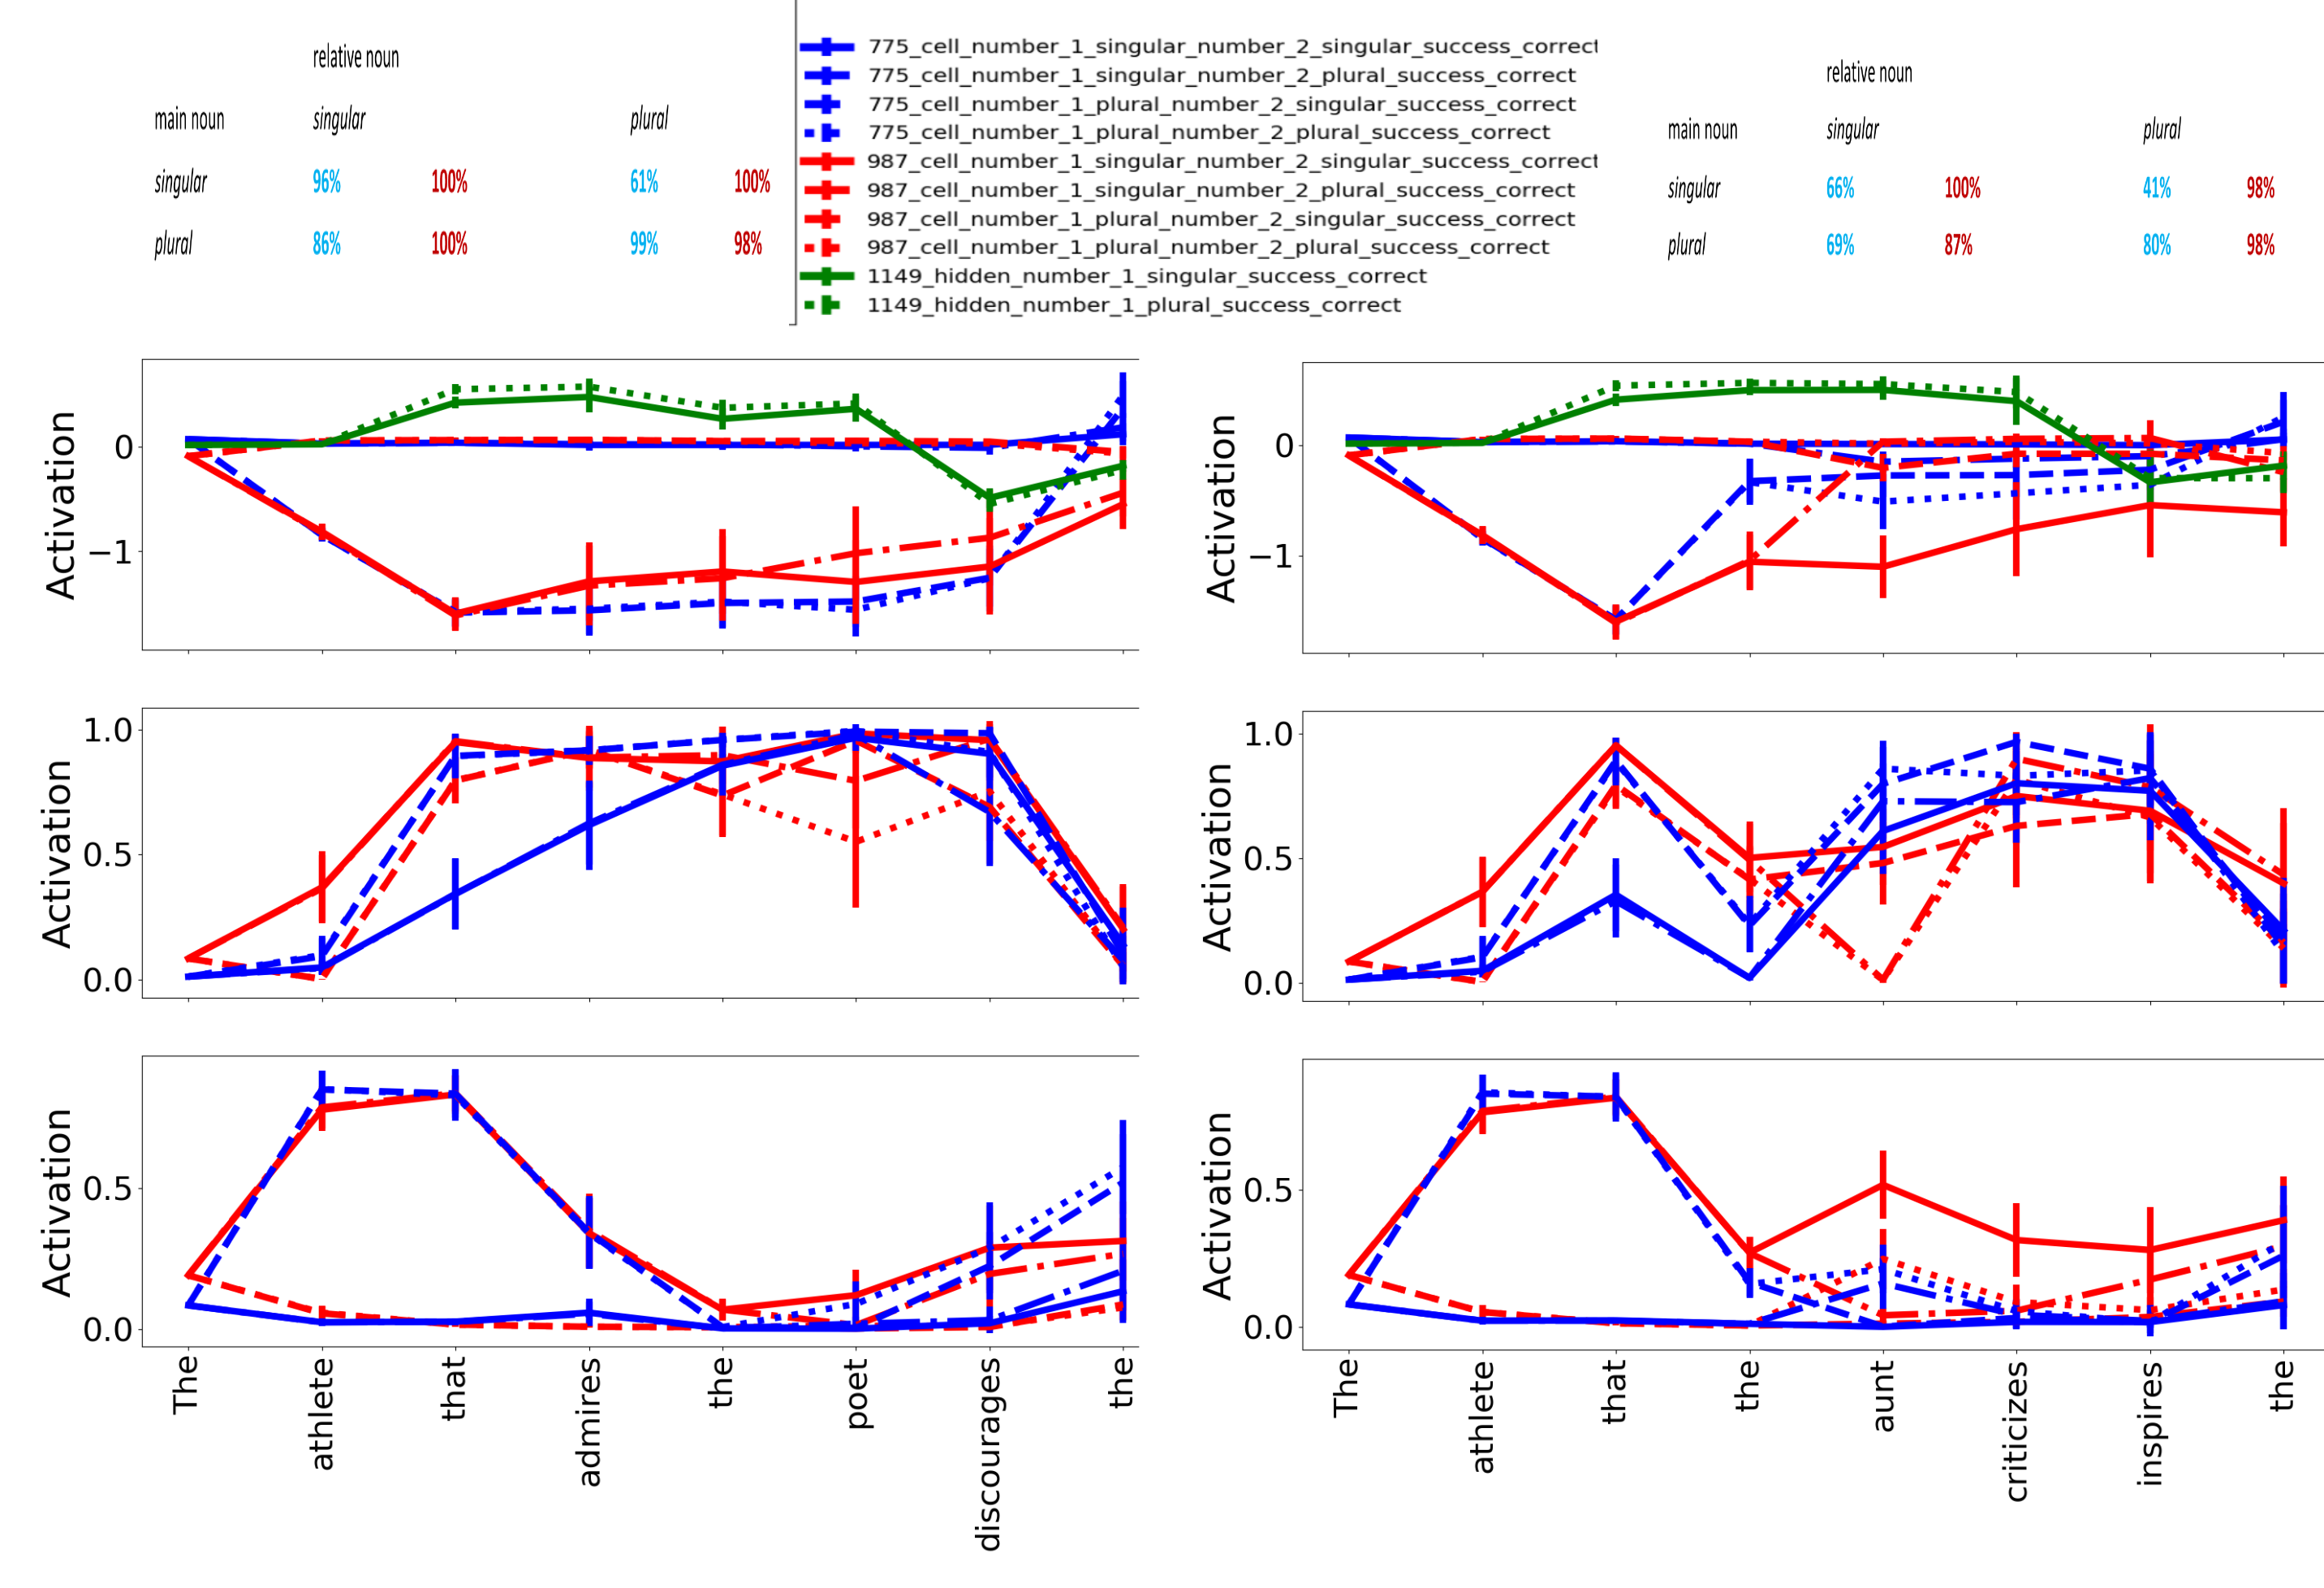
\includegraphics[width=\textwidth]{Figures/Figure8_RC.png}
\caption{Subject-verb agreement in relative clauses: agreement-task accuracy for (A) subject relatives and (B) object relatives. (C \& D) The corresponding cell activations for the number units (775 and 987) and the syntax unit 1149. (E \& F) The corresponding forget-gate activity and (G \& H) input-gate activity of the number units. }
\end{figure*}

\begin{figure}[b]
\centering
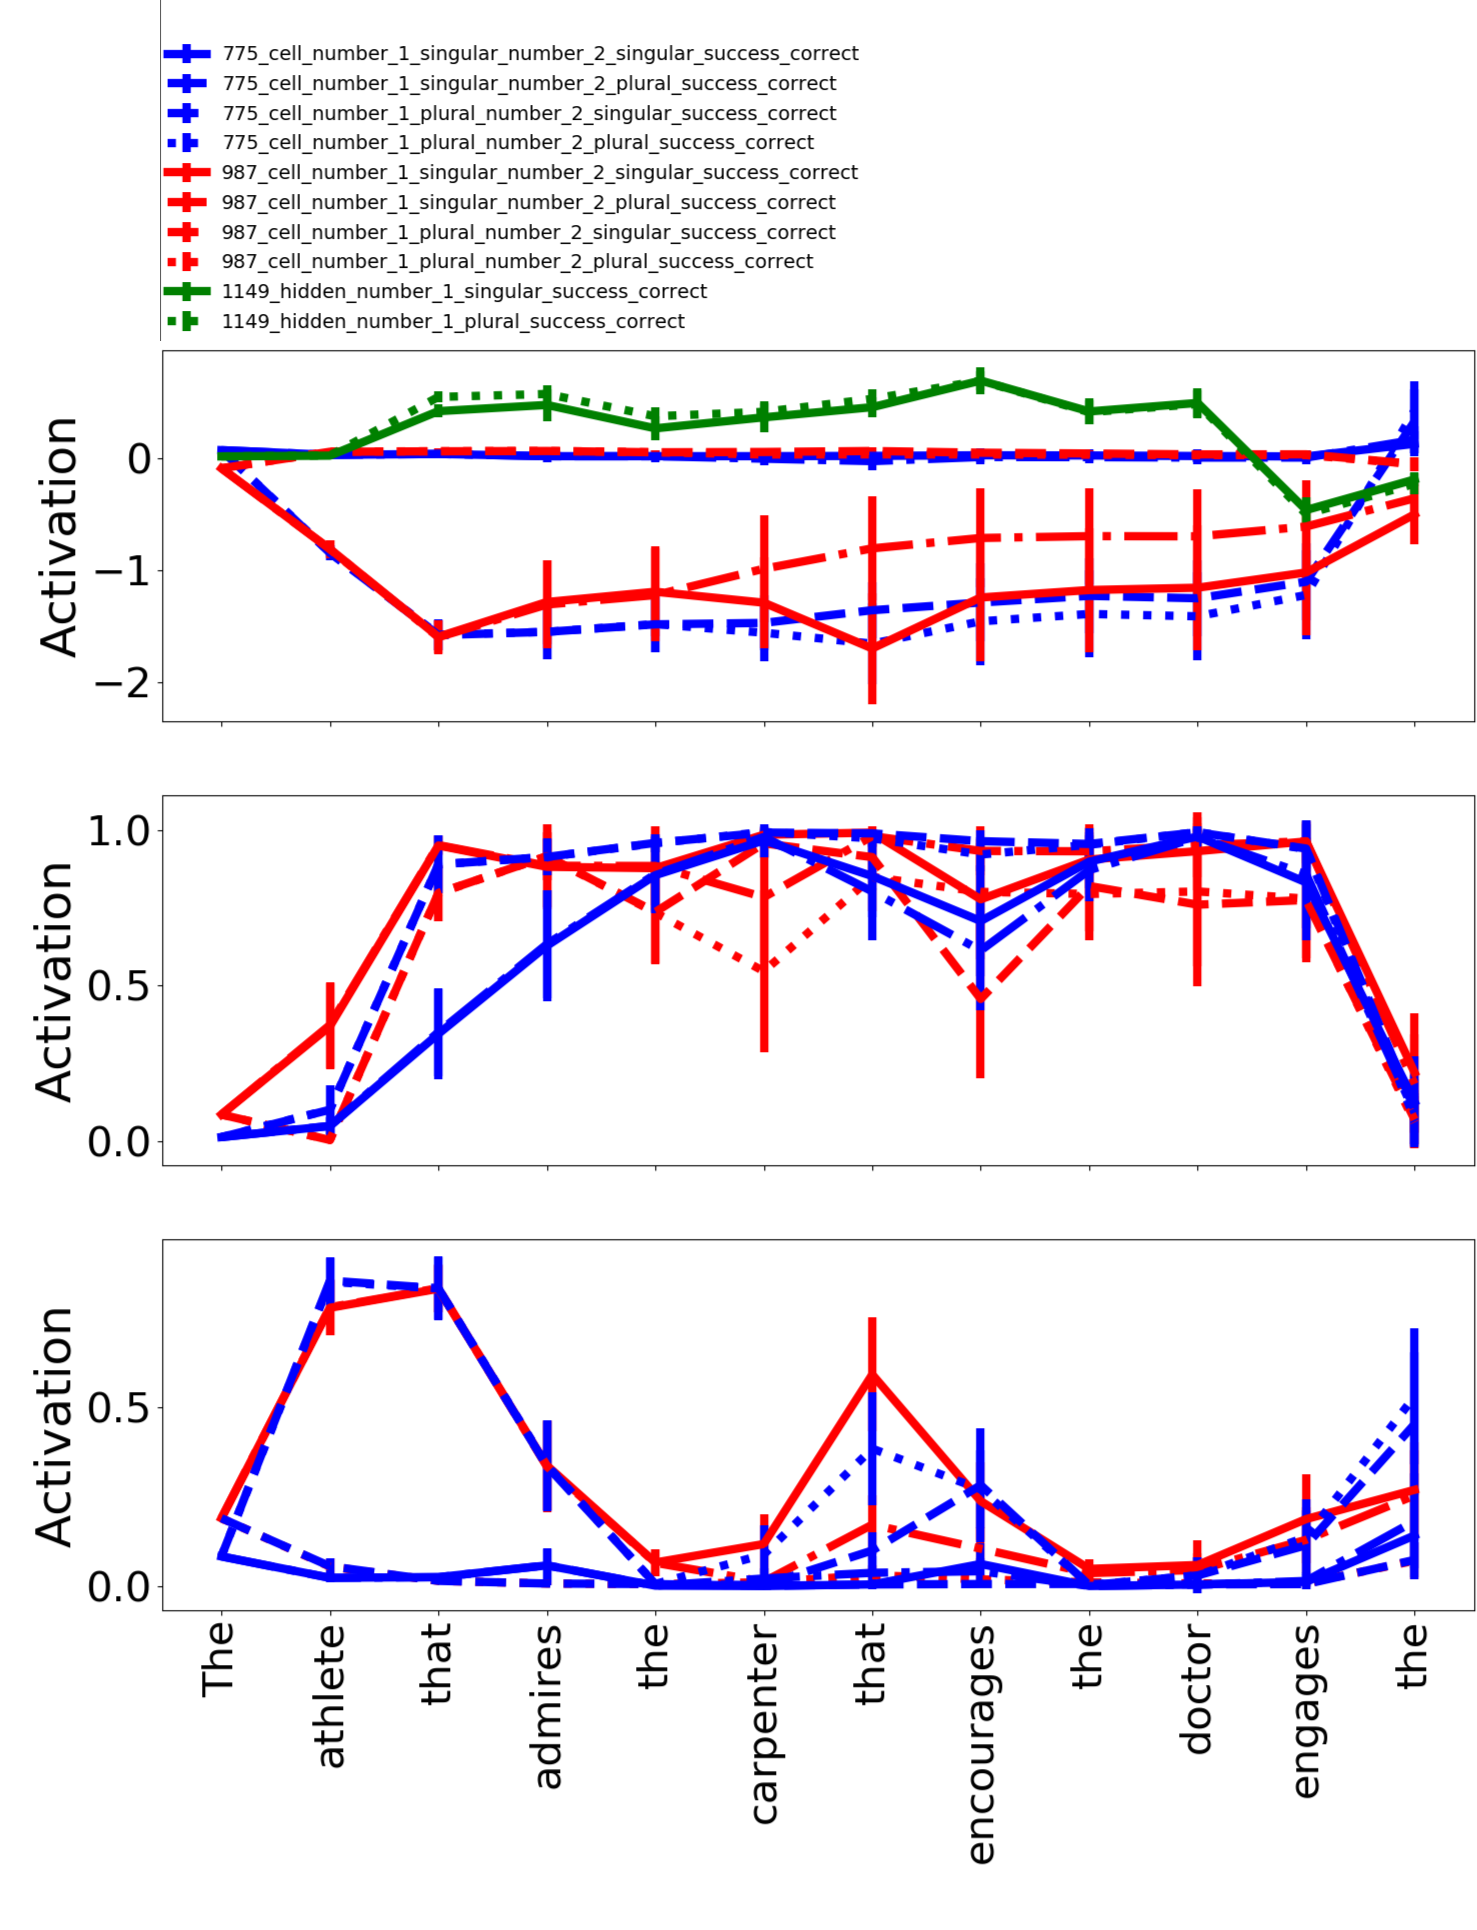
\includegraphics[width=\linewidth]{Figures/Figure9_doubleRC.png}
\caption{Processing of subject relatives with double embeddings. (A) Cell activity of the number and syntax units (775, 987 and 1149) (B) The corresponding forget-gate and (C) input-gate activity.}
\end{figure}

The processing of sentences with relative clauses (RCs) is of particular interest as an NA-task given the presence of another verb before that of the main subject-verb dependency. This section explores number agreement in several types of sentences with RCs. In particular, it compares network behavior and the underlying dynamics of the LR-number units of the NA-task, suggesting an interesting correspondence between the two.

Figure X summarizes the behavioral results of the network on the subjrel (panel A) and objrel (panel B) NA-tasks. We highlight three effects in these results: (1) network performance on the subjrel NA-task is higher compared to the objrel task \textcolor{red}{add stats}; (2) in both subjrel and objrel NA-tasks, network performance was higher in the congruent (main diagonal) than in the incongruent cases (off-diagonal values): $ACC^subjrel_{SS}<ACC^subjrel_{SP}, ACC^subjrel_{PS}<ACC^subjrel_{PP}$ \textcolor{red}{add stats}; (3) When the subject is singular, more errors are made by the network compared to plural: $ACC^objrel{SS}<ACC^objrel{PP}, ACC^objrel{SP}<ACC^objrel{PS}$. Interestingly, these three effects were reported in psycholinguistic studies in humans - human performance is known to be higher in the case of subject compared to object RC (cite), more errors are made by humans in the presenece of an interfering noun (cite), and when the subject is singular (cite). These results are in accordance with similar studies comparing human and machine performance (cite - eg, Linzen 2018), and extend them to the various number conditions.

Panels C \& D in figure X show the corresponding cell and gate (input and forget) dynamics during the processing of subject and object RCs, respectively. Qualitatively, the three effects described above for the behavioral results are reflected in the underlying gate and cell dynamics. Following the same order as above: (1) cell and forget-gate activity preserve a relatively constant value during the processing of subject relatives until the main verb, compared to object RCs, suggesting a more reliable encoding of number information; (2) Cell and forget-gate activity in the incongruent conditions are more perturbated by the inferering noun compared to the corresponding incongruent condition; Similarly, (3) Cell and forget gate activity of unit 988 are more perturbated by the inferering noun compared to that of unit 776 \textcolor{red}{clarify}. Taken together, these dynamics suggest a mechanical explanation for the performance - remarkebly poor in the case of object relatives - of the LSTM language model.

Finally, we look into number-agreement encoding by the LR-number units, and into the encoding of embedded phrases by unit 1150 during the processing of highly demanding sentences with two embedded subject RC (double-subjrel). Figure X shows cell and gate dynamics during the processing of such sentences \textcolor{red}{add behavioral results}. Qualitatively, the forget- and input-gate activity of both LR-number units exhibit the expected dynamics discussed in previous sections (Figure 1B). In addition, the activity of the syntax unit seems to clearly follow the structure of the long-range dependency. One exception is the response of the number units to the relativizer 'that', which generates an increase in cell activation as a result of the opening of the input gate after its presentaiton to the network (see also Figure X). However, this increase in cell activity after a relativizer seems appropriate - to avoid gradual leakage and forgetting of the stored number information in the cell over time, the relativizer seems to signal to the LR-number unit that an embedded phrase is coming before the main verb, thus making the range of the subject-verb dependency even longer. In other words, the language model seems to have learned to make use of the relativizer 'that' for reliable encoding of number information in the case of exceptionally long-range dependnecies as in the case of RCs.
